\chapter{Methods: decay-rate prescriptions across an ensemble of thermodynamic trajectories and bolometric luminosity}\label{ch:methods}

This chapter describes how the results of Chapter~\ref{ch:results} were obtained.
The calculation is a chain of four stages.
First, we construct an ensemble of 512 parametrized thermodynamic trajectories that covers the conditions found in the ejecta of neutron star mergers (Sec.~\ref{sec:methods_trajectories}).
Second, every trajectory is evolved with the nuclear reaction network WinNet~\cite{reichert_nuclear_2023} for three different sets of $\beta^-$- and $\alpha$-decay rates, which differ only in the prescription adopted for the nuclei without measured half-lives.
Third, the radioactive heating rate of each run is computed from its abundances and separated by decay channel and by nucleus.
Fourth, the heating rates are used as input of a kilonova model to obtain light curves.
The theory behind each stage was developed in Chapters~\ref{chap:BNMS}--\ref{ch:rad_models}.

The work follows and extends the study published in Ref.~\cite{hernandez_porras_features_2027}.
In that study the impact of the decay-rate prescriptions was compared along a single trajectory of the dynamical ejecta, and their robustness was tested with 120 parametric trajectories restricted to cold, very neutron-rich conditions ($Y_e\leq0.20$, $s\leq10\,k_B$ per baryon).
Here the ensemble is the central object.
It is more than four times larger, it extends to the electron fractions, entropies and velocities of the shock-heated and post-merger ejecta, and its initial state is computed with a complete equation of state instead of an ion-dominated approximation.
Table~\ref{tab:paper_vs_thesis} lists the differences between the two setups.
Since every trajectory is evolved with each rate set, all comparisons between prescriptions are made trajectory by trajectory.

\begin{table}[t]
\caption{Setup of this work compared with that of Ref.~\cite{hernandez_porras_features_2027}.\label{tab:paper_vs_thesis}}\vspace{0.25em}
\centering{\small
\begin{tabular}{@{}p{0.2\textwidth}p{0.365\textwidth}p{0.365\textwidth}@{}}
\toprule
 & Ref.~\cite{hernandez_porras_features_2027} & This work \\
\midrule
Trajectories & one hydrodynamic trajectory; 120 parametric trajectories & 512 parametric trajectories \\
Parameters & $(Y_{e,0},s_0,\tau)$ at $T_0=7\,\mathrm{GK}$ & $(Y_{e,0},s_0,v_\infty)$ at $T_0=10\,\mathrm{GK}$ \\
Ranges & $Y_{e,0}\in[0.01,0.20]$,& $Y_{e,0}\in[0.04,0.42]$,\\
&$s_0\in[1,10]$,&$s_0\in[1,49]$,\\
&$\tau\in[0.2,2]\,\mathrm{ms}$&$v_\infty\in[0.01,0.49]\,c$ \\
Initial density & Sackur--Tetrode entropy of the ions with a 47-isotope NSE & total entropy (ions in NSE with 7852 nuclei, $e^\pm$, photons) \\
Heating rate & $Q$-values from ENSDF, abundances from the network & rates, $Q$-values and neutrino fractions of the network itself \\
\bottomrule
\end{tabular}}
\end{table}

%==========================================================================================
\section{Parametric thermodynamic trajectories}\label{sec:methods_trajectories}
%==========================================================================================

The network equation (Eq.~\ref{eq:network}) needs the density history $\rho(t)$ of the fluid element, its initial composition and its initial entropy.
In hydrodynamic simulations these are recorded by tracer particles.
Here we use instead the parametric approach of Lippuner and Roberts~\cite{lippuner_r-process_2015}, also adopted in recent surveys of r-process conditions~\cite{kuske_complete_2025}, in which a trajectory is defined by a small number of physical parameters.

\subsection{Parametrization of the expansion}\label{sec:methods_expansion}

Each trajectory is defined by three parameters given at a reference temperature $T_0=10\,\mathrm{GK}$: the electron fraction $Y_{e,0}$, the entropy per baryon $s_0$ and the asymptotic expansion velocity $v_\infty$.
At $T_0$ the matter is in nuclear statistical equilibrium (NSE, Sec.~\ref{sec:nse}), so its composition is a function of $(\rho,T,Y_e)$ and no further information is required.
The density follows Eq.~\ref{eq:homol},
\begin{equation}\label{eq:traj_density}
  \rho(t)=
  \begin{cases}
    \rho_0\,e^{-t/\tau} & t\leq3\tau,\\[2pt]
    \rho_0\left(\dfrac{3\tau}{e\,t}\right)^{3} & t\geq3\tau,
  \end{cases}
\end{equation}
which is continuous together with its first derivative at $t=3\tau$.
The fluid element is assigned an initial radius $R_0=50\,\mathrm{km}$, and mass conservation in a comoving volume, $\rho R^3=\rho_0R_0^3$, gives
\begin{equation}\label{eq:traj_radius}
  R(t)=
  \begin{cases}
    R_0\,e^{t/3\tau} & t\leq3\tau,\\[2pt]
    R_0\,\dfrac{e\,t}{3\tau} & t\geq3\tau.
  \end{cases}
\end{equation}
The velocity $\mathrm{d}R/\mathrm{d}t$ therefore grows from $R_0/(3\tau)$ at $t=0$ to the constant value $eR_0/(3\tau)$ of the homologous branch, which we identify with $v_\infty$.
The expansion timescale is then fixed by the velocity,
\begin{equation}\label{eq:tau_vinf}
  \tau=\frac{e\,R_0}{3\,v_\infty}.
\end{equation}
The network depends on the expansion only through $\rho(t)$, so $R_0$ has no effect other than setting the correspondence between $\tau$ and $v_\infty$.
We prefer $v_\infty$ as the parameter because it is the quantity reported by merger simulations and the one that enters the kilonova model.

\subsection{Initial density from the entropy}\label{sec:methods_rho0}

The initial density $\rho_0$ is not a free parameter.
It is the density at which matter with electron fraction $Y_{e,0}$ and temperature $T_0$ has the entropy $s_0$,
\begin{equation}\label{eq:rho0_condition}
  s_{\rm ion}(T_0,\rho_0,Y_{e,0})+s_{e^\pm}(T_0,\rho_0Y_{e,0})+s_\gamma(T_0,\rho_0)=s_0 ,
\end{equation}
where the three terms are the entropies per baryon, in units of $k_B$, of the nuclei, of the electron--positron gas and of the photons.

\paragraph{Ions.}
The composition is obtained from the Saha equation (Eq.~\ref{eq:saha}) for the 7852 nuclei of the WinNet nuclear data table, which provides the mass excesses, ground-state spins and partition functions $G_i(T)$.
The two constraints of Eq.~\ref{eq:conservation} are solved for the degeneracy parameters of the free neutrons and protons with a Newton--Raphson iteration.
Each species is a non-degenerate ideal gas with internal degeneracy $g_iG_i(T)$ (Appendix~\ref{ap:Detailed_balance}), whose entropy follows from its free energy.
Summing over species\footnote{Coulomb corrections are neglected.},
\begin{equation}\label{eq:s_ion}
  s_{\rm ion}=\sum_iY_i\left[\frac52+\ln\!\left(\frac{g_iG_i}{n_i\Lambda_i^3}\right)+\frac{\mathrm{d}\ln G_i}{\mathrm{d}\ln T}\right],
\end{equation}
with $n_i=\rho N_AY_i$ and $\Lambda_i$ the thermal wavelength defined in Sec.~\ref{sec:saha}.
The first two terms are the Sackur--Tetrode entropy of each species, and the last one is the contribution of the thermally populated excited states.

\paragraph{Electrons, positrons and photons.}
The entropy of the $e^\pm$ gas is taken from the Helmholtz equation of state~\cite{timmes_accuracy_2000}, which is valid for arbitrary degeneracy and includes the thermal pairs.
At fixed temperature it is a function of $\rho Y_e$ alone, so it is tabulated once and interpolated with splines.
The photons contribute
\begin{equation}\label{eq:s_gamma}
  s_\gamma=\frac{4aT^3}{3\,\rho N_Ak_B}\simeq1.21\times10^{5}\,\frac{T_9^{3}}{\rho\,[\mathrm{g\,cm^{-3}}]},
\end{equation}
with $a$ the radiation constant.

\paragraph{Solution.}
At fixed $T_0$ and $Y_{e,0}$ the total entropy decreases monotonically with density, so Eq.~\ref{eq:rho0_condition} has a single root.
This is a substantial change with respect to Ref.~\cite{hernandez_porras_features_2027}, where $\rho_0$ was obtained from the Sackur--Tetrode entropy of a gas of mean mass number $\bar A$.
That approximation is adequate when the ions dominate the entropy, but it fails in the larger parameter space explored here.
For $s_0\geq35$ the ions carry on average only $30\%$ of the entropy, while the $e^\pm$ pairs carry $44\%$ and the photons $26\%$.
For $s_0<5$ the ions carry $89\%$.

Figure~\ref{fig:rho0_map} shows the resulting $\rho_0(s_0,Y_{e,0})$.
Across the ensemble $\rho_0$ spans more than five orders of magnitude, from $9.0\times10^{6}$ to $2.3\times10^{12}\,\mathrm{g\,cm^{-3}}$, with a median of $2.3\times10^{7}\,\mathrm{g\,cm^{-3}}$, and it is controlled almost entirely by $s_0$.
The composition at $T_0$ changes accordingly.
For $s_0\geq10$ the matter consists of free nucleons and $\alpha$ particles, with less than $2\times10^{-4}$ of the mass in heavier nuclei.
Only at the lowest entropies, $s_0\lesssim5$, are heavy nuclei already abundant at $10\,\mathrm{GK}$.

%%%%%%%%%%%%%%%%%  figure: rho0 map  %%%%%%%%%%%%%%%%%
\begin{figure}[t]
  \centering
  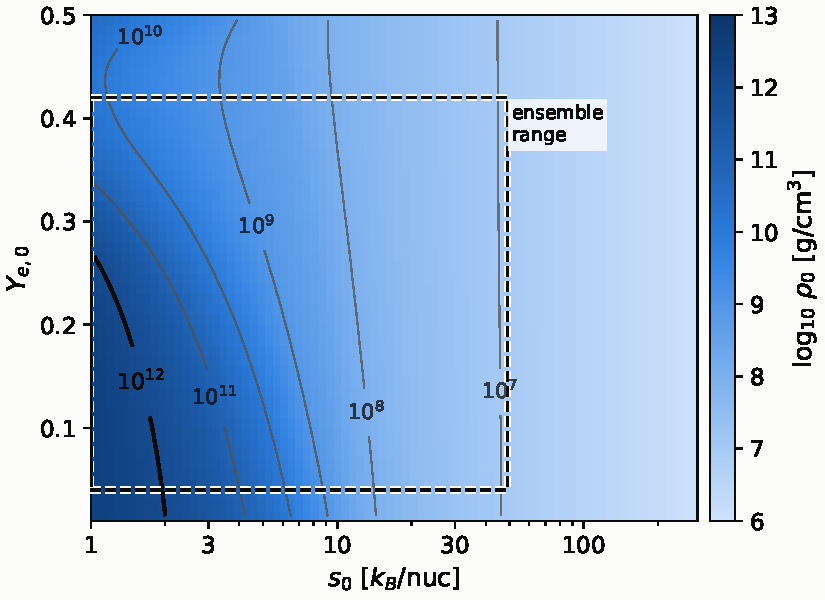
\includegraphics[width=0.8\textwidth]{Figures/rho0_map_T10GK.pdf}
  \caption{Initial density $\rho_0$ that satisfies Eq.~\ref{eq:rho0_condition} at $T_0=10\,\mathrm{GK}$, as a function of the entropy per baryon $s_0$ and the electron fraction $Y_{e,0}$. The contour marks $\rho_0=10^{12}\,\mathrm{g\,cm^{-3}}$, above which the non-degenerate treatment of the nucleons is no longer reliable.}
  \label{fig:rho0_map}
\end{figure}

Equation~\ref{eq:s_ion} assumes Maxwell--Boltzmann statistics for the nucleons.
At $T_0$ this requires $\rho\ll10^{12}\,\mathrm{g\,cm^{-3}}$ because above that density the free neutrons become degenerate and nuclear interactions can no longer be neglected.
A second, smaller inconsistency is that the NSE composition of the network is restricted to its 6757 nuclei and includes screening corrections~\cite{reichert_nuclear_2023}.
Since the network recomputes the NSE composition when it starts (Sec.~\ref{sec:methods_start}), these differences affect only the value of $\rho_0$ assigned to a given $s_0$.

\subsection{Sampling of the parameter space}\label{sec:methods_sampling}

The three parameters are sampled uniformly in the ranges
\begin{equation}\label{eq:ranges}
  0.04\leq Y_{e,0}\leq0.42,\qquad 1\leq s_0\leq49\ k_B\,\mathrm{baryon^{-1}},\qquad 0.01\leq v_\infty/c\leq0.49 .
\end{equation}
The ranges were chosen to contain the conditions of all the ejecta components described in Chapter~\ref{chap:BNMS}.
These include the cold and very neutron-rich tidal ejecta ($Y_e\lesssim0.15$), the shock-heated ejecta with electron fractions up to $\approx0.4$, both with asymptotic velocities of $0.1$--$0.3\,c$, and the slower post-merger outflows~\cite{radice_dynamical_2016,radice_binary_2018,radice_dynamics_2020,shibata_merger_2019}.
The entropies of $10$--$30\,k_B$ per baryon typical of merger ejecta lie in the middle of the adopted range.
The ranges also cross the boundary $Y_e\approx0.25$ that separates lanthanide-rich from lanthanide-poor nucleosynthesis (Sec.~\ref{sec:n_to_seed}): 283 trajectories lie below it, and 148 have $Y_{e,0}<0.15$, where fission cycling is expected (Sec.~\ref{sec:fission}).
By Eq.~\ref{eq:tau_vinf} the velocity range corresponds to expansion timescales between $0.31$ and $14.5\,\mathrm{ms}$.
Since the sampling is uniform in $v_\infty$, it is not uniform in $\tau$.
The median is $0.60\,\mathrm{ms}$ and $90\%$ of the trajectories lie between $0.33$ and $4.4\,\mathrm{ms}$.
For comparison, the survey of Ref.~\cite{lippuner_r-process_2015} covered $0.01\leq Y_e\leq0.50$, $1\leq s\leq100$ and $0.1\leq\tau\leq500\,\mathrm{ms}$.

The points are drawn from a scrambled Sobol sequence of $2^{9}=512$ points in three dimensions, generated with SciPy from a fixed seed.
This was done because a low-discrepancy sequence fills the box more evenly than independent random draws.
In particular, the first $2^m$ points of a Sobol sequence are stratified in each coordinate.
When the range of any parameter is divided into 512 equal intervals, each interval contains exactly one trajectory.
For the same reason the number of points is kept a power of two.
Figure~\ref{fig:ensemble} shows the projections of the ensemble.

%%%%%%%%%%%%%%%%%  figure: ensemble coverage  %%%%%%%%%%%%%%%%%
\begin{figure}[t]
  \centering
  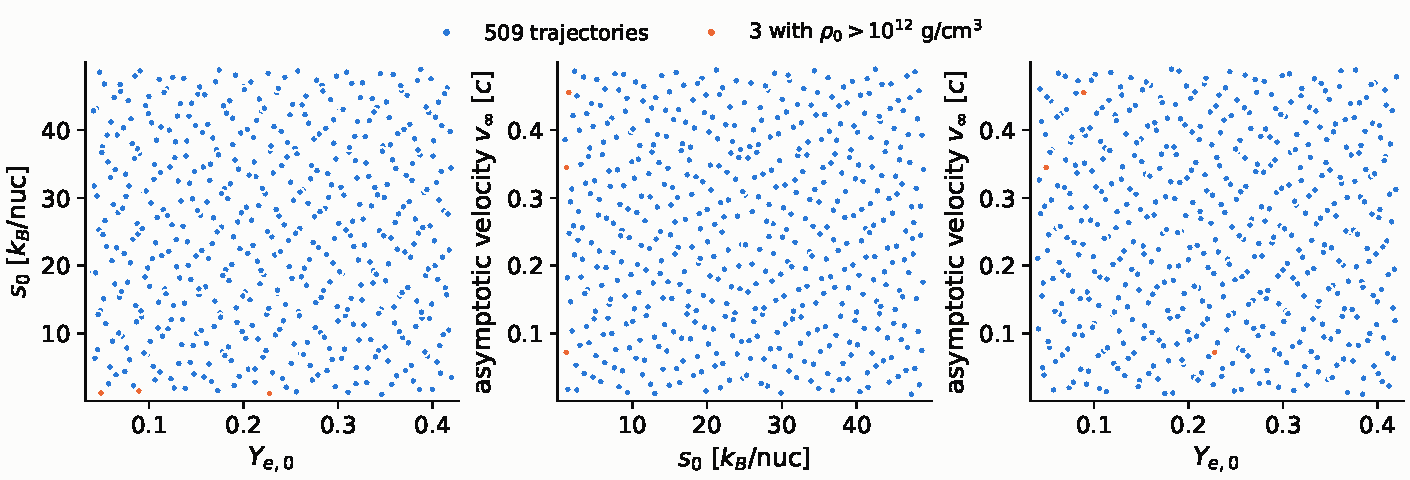
\includegraphics[width=1\textwidth]{Figures/ensemble_projections.pdf}
  \caption{Projections of the ensemble of 512 trajectories on the three coordinate planes of the parameter space of Eq.~\ref{eq:ranges}.}
  \label{fig:ensemble}
\end{figure}

It is important to state what this ensemble represents.
It is a uniform design over a box, built to measure how the effect of the decay-rate prescriptions depends on the thermodynamic conditions.
It is not a model of the ejecta of a particular merger.
At this point no mass is attached to the trajectories, and the box contains combinations of parameters, such as $v_\infty\approx0.5\,c$ with $s_0\approx1$, that no simulation produces in significant amounts.
All ensemble statistics quoted in this thesis (medians, percentile bands, means) are therefore statistics over the box with equal weight per trajectory.

\subsection{Trajectory files and starting point of the network}\label{sec:methods_start}

Each trajectory is written as a table of time, temperature, density, radius and electron fraction, on 400 points from $t=0$ to $t=1\,\mathrm{s}$, logarithmically spaced from $10^{-3}\tau$ and including $t=3\tau$ exactly.
Beyond the last point WinNet continues the expansion ballistically with the velocity of the last points~\cite{korobkin_astrophysical_2012,reichert_nuclear_2023}.
The electron fraction column is only the initial value, because the network evolves $Y_e$ with its weak rates (Eq.~\ref{eq:dYe_network}).
Figure~\ref{fig:trajectories_rho} shows $\rho(t)$ and Figure~\ref{fig:trajectories_T_Ye} the temperature and electron fraction for a sample of trajectories for each prescription.
The temperature is recovered from the entropy, which evolves according to Eq.~\ref{eq:entropy_eq} (Sec.~\ref{sec:self_heating}).
From Figure~\ref{fig:trajectories_T_Ye} we can draw two important conclusions.
First, if the initial density is high enough, the temperature will rise on timescales of seconds due to self-heating.
Second, if the ejecta have low initial density, low electron fraction and high asymptotic velocity, the synthesis will be dominated by the $\beta^{-}$ decay of free neutrons, so the final $Y_e$ corresponds to ejecta composed mostly of hydrogen.
Such conditions are rare in a real merger.


%%%%%%%%%%%%%%%%%  figure: trajectories  %%%%%%%%%%%%%%%%%
\begin{figure}[t]
  \centering
  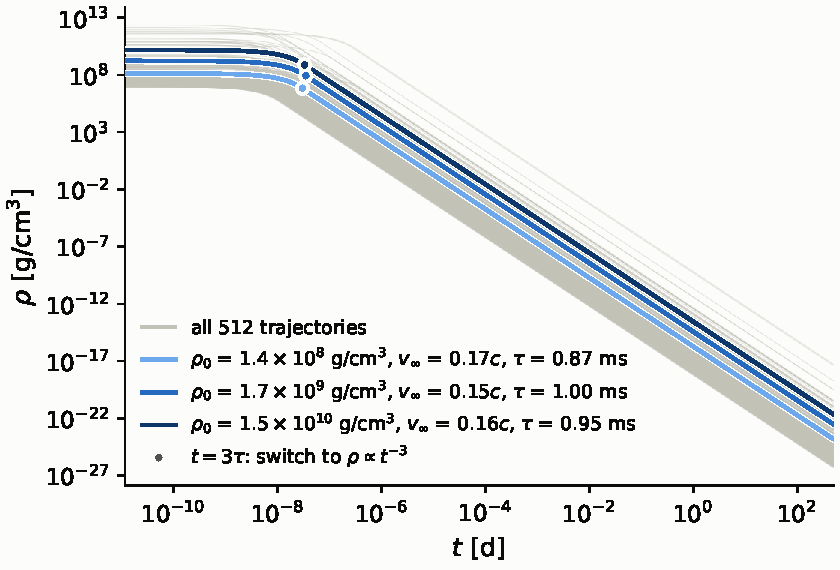
\includegraphics[width=0.9\textwidth]{Figures/run_density.pdf}
  \caption{Densities (Eq.~\ref{eq:traj_density}) as functions of time for a sample of trajectories of the ensemble.}
  \label{fig:trajectories_rho}
\end{figure}
\begin{figure}[h]
  \centering
  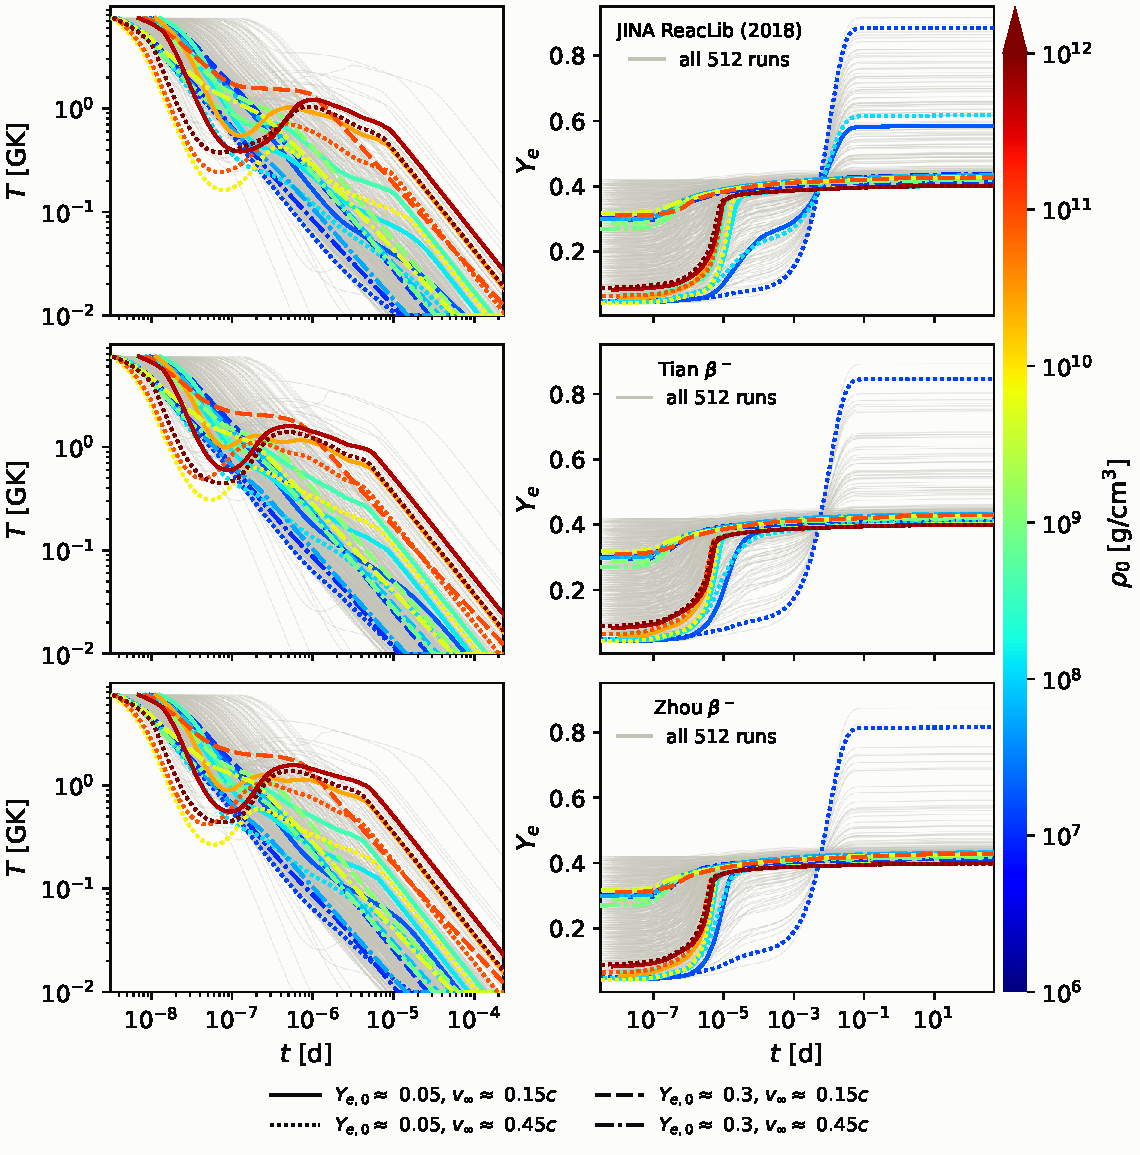
\includegraphics[width=0.9\textwidth]{Figures/run_T_Ye.pdf}
  \caption{Temperature (Eq.~\ref{eq:T_general}) and electron fraction $Y_e$ as functions of time for a sample of trajectories of the ensemble.}
  \label{fig:trajectories_T_Ye}
\end{figure}

%==========================================================================================
%\section{Nuclear reaction network}\label{sec:methods_network}
%==========================================================================================

\section{Nuclear reaction network configuration}\label{sec:methods_winnet}

All calculations were performed with WinNet~\cite{reichert_nuclear_2023}, which integrates the network equation (Eq.~\ref{eq:network}) with an implicit Euler scheme.
The setup, summarized in Table~\ref{tab:winnet_setup}, is that of the dynamical-ejecta example distributed with the code, with the changes described below.
It is identical for all trajectories and all rate sets, except for the decay rates discussed in Sec.~\ref{sec:methods_rates}.

\begin{table}[t]
\caption{Configuration of the network calculations.\label{tab:winnet_setup}}\vspace{0.25em}
\centering{\small
\begin{tabular}{@{}p{0.27\textwidth}p{0.67\textwidth}@{}}
\toprule
Ingredient & Choice \\
\midrule
Nuclei & 6757, from free nucleons to $Z=110$ \\
Nuclear data & masses, spins and partition functions of the WinNet table \texttt{winvne\_v2.0} \\
Reaction rates & JINA ReacLib~\cite{cyburt_jina_2010} (file \texttt{Reaclib\_18\_9\_20} distributed with WinNet) \\
Weak rates at high $T$ & Langanke and Mart\'inez-Pinedo~\cite{langanke_rate_2001}; replaced by the experimental rates below $T_9=10^{-2}$ \\
$\beta^-$ and $\alpha$ decays & measured rates, complemented by one of the three sets of Table~\ref{tab:rate_sets} \\
Neutron-induced fission & Panov et al.~\cite{panov_neutron-induced_2010} \\
$\beta$-delayed fission & Mumpower et al.~\cite{mumpower_2022} \\
Spontaneous fission & Khuyagbaatar~\cite{khuyagbaatar_spontaneous_2020} with the barriers of M\"oller et al.~\cite{moller_fission_2015} \\
Fission fragments & Panov et al.~\cite{panov_could_2001} \\
Screening & Kravchuk and Yakovlev~\cite{kravchuk_strong_2014} \\
Start & $T_{\rm start}=7.5\,\mathrm{GK}$, composition in NSE \\
NSE $\leftrightarrow$ network & network below $7\,\mathrm{GK}$; NSE again above $8\,\mathrm{GK}$ \\
Temperature & from the entropy (self-heating), Helmholtz equation of state~\cite{timmes_accuracy_1999,timmes_accuracy_2000} \\
Neutrino losses & tabulated mean neutrino energies~\cite{brown_endfb-viii0_2018} for 1384 nuclei, $40\%$ of the $Q$-value otherwise.\\
Heating active below & $\rho=10^{11}\,\mathrm{g\,cm^{-3}}$ \\
Rates frozen below & $T_9=10^{-2}$ \\
Expansion after $1\,\mathrm{s}$ & ballistic, $\rho\propto t^{-3}$ \\
Final time & $4.32\times10^{7}\,\mathrm{s}$ (500 days) \\
\bottomrule
\end{tabular}}
\end{table}

The network contains 6757 nuclei.
JINA ReacLib has 78\,910 rates, of which 4861 are $\beta^-$ decays and 1439 are $\alpha$ decays; only 1041 and 256 of them, respectively, are from experiments.
The remaining decay rates are theoretical.
Fission is included in its three modes (Sec.~\ref{sec:fission}), with the fragment distribution of Panov et al.~\cite{panov_could_2001} in all calculations.

The calculation starts at $7.5\,\mathrm{GK}$ with the NSE composition (Sec.~\ref{sec:methods_start}).
The composition is kept in NSE until the temperature falls below $7\,\mathrm{GK}$, where the full network takes over.
NSE is assumed again if the temperature rises above $8\,\mathrm{GK}$.
The entropy is evolved with Eq.~\ref{eq:entropy_eq}~\cite{freiburghaus_r-process_1999}, and the temperature is obtained at every step by inverting the Helmholtz equation of state~\cite{timmes_accuracy_2000} at the density of the trajectory.
The term $\dot q_{\rm ext}$ of Eq.~\ref{eq:qnu} uses the mean neutrino energy of each $\beta$ decay where it is known from evaluated data~\cite{brown_endfb-viii0_2018}, and a fraction $\chi_\nu=0.4$ of the $Q$-value for all other nuclei.
Nuclear heating is applied only once the density is below $10^{11}\,\mathrm{g\,cm^{-3}}$, where the assumption that neutrinos escape freely is justified.
Below $T_9=10^{-2}$, the lower limit of validity of the ReacLib fits, all rates are frozen.
In our runs this limit is reached within a few seconds, so the late-time evolution, which is the one relevant for the kilonova, proceeds with constant decay rates and is the linear problem described in Sec.~\ref{sec:decay_chains}.

Each run ends at 500 days.
The abundances of all nuclei are stored every 100 time steps, which gives 54 to 57 snapshots per run, approximately equally spaced in $\log t$; the global quantities (temperature, entropy, $Y_e$, energy generation and neutrino losses) are stored every 10 steps.

\subsection{Decay-rate prescriptions}\label{sec:methods_rates}

The three sets of calculations differ only in the $\beta^-$- and $\alpha$-decay rates of the nuclei without experimental half-lives (Table~\ref{tab:rate_sets}).
The measured rates are the same in the three sets, and so is every other reaction.

\begin{table}[t]
\caption{Rate sets. Each set was run for the 512 trajectories. The last two columns give the number of $\beta^{-}$ and $\alpha$ decay rates. \label{tab:rate_sets}}\vspace{0.25em}
\centering{\small
\begin{tabular}{@{}lllcc@{}}
\toprule
Set & $\beta^-$ & $\alpha$ & $N_{\beta^-}$ & $N_\alpha$ \\
\midrule
ReacLib & FRDM+QRPA~\cite{moller_new_2003} & ReacLib, Viola--Seaborg~\cite{dong_new_2005} & 4861 & 1439 \\
Tian    & Tian et al.~\cite{tian_empirical_2025} & NMHF~\cite{sharma_new_2021} & 5181 & 2933 \\
Zhou    & Zhou et al.~\cite{zhou_empirical_2017} & NMHF~\cite{sharma_new_2021} & 4884 & 2933 \\
\bottomrule
\end{tabular}}
\end{table}

The theoretical $\beta^-$ rates from ReacLib come from the quasiparticle random-phase approximation on top of the finite-range droplet model (FRDM+QRPA)~\cite{moller_new_2003}.
The $\alpha$ decays of the library are complemented with additional rates from the Viola--Seaborg formula~\cite{viola_nuclear_1966},
\begin{equation}\label{eq:viola_seaborg}
  \log_{10}T_{1/2}=\frac{aZ+b}{\sqrt{Q_\alpha}}+cZ+d+h_{\log},
\end{equation}
with the parameters of Dong and Ren~\cite{dong_new_2005} and a hindrance term $h_{\log}$ that depends on the parity of $Z$ and $N$, as implemented in WinNet~\cite{reichert_nuclear_2023}.


\paragraph{Empirical formulae for $\beta^-$ decay.}
The two alternative sets replace the FRDM+QRPA rates by empirical formulae.
Both start from Sargent's law, $T_{1/2}\propto Q_\beta^{-5}$, and add corrections fitted to the measured half-lives.
The formula of Zhou et al.~\cite{zhou_empirical_2017} reads
\begin{equation}\label{eq:zhou}
  \ln T_{1/2}=a_6+\left(\alpha^2Z^2-5-a_7\frac{N-Z}{A}\right)\ln\left(Q_\beta-a_8\delta\right)+a_9\alpha^2Z^2+\frac13\alpha^2Z^2\ln A-\alpha Z\pi+S(Z,N),
\end{equation}% CHECK the signs and the base of the logarithm against the original paper (taken from papers that quote it).
where $\alpha$ is the fine-structure constant, $\delta=(-1)^N+(-1)^Z$ accounts for pairing, and the terms in $\alpha Z$ account for the Coulomb field of the daughter nucleus.
The formula of Tian et al.~\cite{tian_empirical_2025} adds the dependence of the total Gamow--Teller strength on the neutron excess,
\begin{equation}\label{eq:tian}
  \ln T_{1/2}=a_1-a_2\ln\left(Q_\beta+m_ec^2+a_3\delta\right)+S(Z,N)-a_8\ln\left(Ze^{-N/Z}+Ne^{-Z/N}+N-Z\right).
\end{equation}
In both cases $S(Z,N)$ is a shell correction, a sum of Gaussians in $Z$ and $N$ centered near the closed shells, and the parameters $a_k$ are fitted to the measured $\beta^-$ half-lives; their values are given in the original references.
The $Q$-values were calculated from the mass differences, using the same mass table as the reaction network.

\paragraph{Empirical formula for $\alpha$ decay.}
In the Tian and Zhou sets the theoretical $\alpha$-decay rates are given by the new modified Horoi formula (NMHF) of Sharma et al.~\cite{sharma_new_2021},
\begin{equation}\label{eq:nmhf}
  \log_{10}T_{1/2}=\left(a\sqrt{\mu}+b\right)\left[\frac{(Z_\alpha Z_d)^{0.6}}{\sqrt{Q_\alpha}}-7\right]+\left(c\sqrt{\mu}+d\right)+e\,I+f\,I^2+g\,l(l+1),
\end{equation}
where $Z_\alpha=2$, $Z_d$ and $A_d$ are the charge and mass numbers of the daughter, $\mu=4A_d/(A_d+4)$ is the reduced mass number, $I=(N-Z)/A$ is the asymmetry of the parent and $l$ is the minimum angular momentum carried by the $\alpha$ particle, fixed by the spins and parities of parent and daughter.
The $\alpha$ prescription therefore changes together with the $\beta^-$ prescription between the reference set and the other two.
This is justified by the result of Ref.~\cite{hernandez_porras_features_2027} that the heating rate is insensitive to the choice of empirical $\alpha$ formula, because the $\alpha$ emitters that dominate the heating have measured half-lives.
The differences between the reference set and the Tian or Zhou sets are thus attributed to the $\beta^-$ rates, and the comparison between Tian and Zhou, which share the $\alpha$ rates, isolates them exactly.

\paragraph{Implementation.}
A constant decay rate is the special case of Eq.~\ref{eq:reaclib} in which only the first coefficient is different from zero,
\begin{equation}\label{eq:a0}
  a_0=\ln\left(\frac{\ln2}{T_{1/2}}\right),\qquad a_1=\dots=a_6=0 .
\end{equation}
For each formula we evaluate $T_{1/2}$ and write a library in ReacLib format in which the theoretical $\beta^-$ and $\alpha$ entries carry the coefficient of Eq.~\ref{eq:a0}, while the entries based on measurements and all other reactions are left untouched.
For nuclei that the formula does not cover, the original ReacLib rate was used.
The additional $\alpha$ decay rates from Viola--Seaborg were used in all the sets as an alternative when NMHF cannot be used.

\paragraph{Validation and limitations.}
Figure~\ref{fig:rate_coverage} shows the regions of the nuclear chart covered by the measurements, by ReacLib and by each formula\footnote{The figure uses an extra $\alpha$ decay prescription that we are not implementing here due to the fact that theoretical $\alpha$ decay rates far from stability do not contribute to the r-process.}, and Fig.~\ref{fig:rate_comparison} compares the formulae with the ReacLib rates and with experiment.
The $\alpha$ formulae reproduce the measured half-lives well.
For $\beta^-$ decay the formula of Tian et al.\ shows larger deviations from experiment than that of Zhou et al., which in turn covers a smaller region of the chart~\cite{hernandez_porras_features_2027}.
An empirical formula has no information on the structure of individual nuclei beyond $Q_\beta$, $Z$ and $N$.
It is designed for the short-lived nuclei far from stability, and it can fail for nuclei close to stability whose decay is hindered by a large spin change.

%%%%%%%%%%%%%%%%%  figures: coverage and comparison (Figs. 3 and 4 of the paper)  %%%%%%%%%%%%%%%%%
\begin{figure}[t]
  \centering
  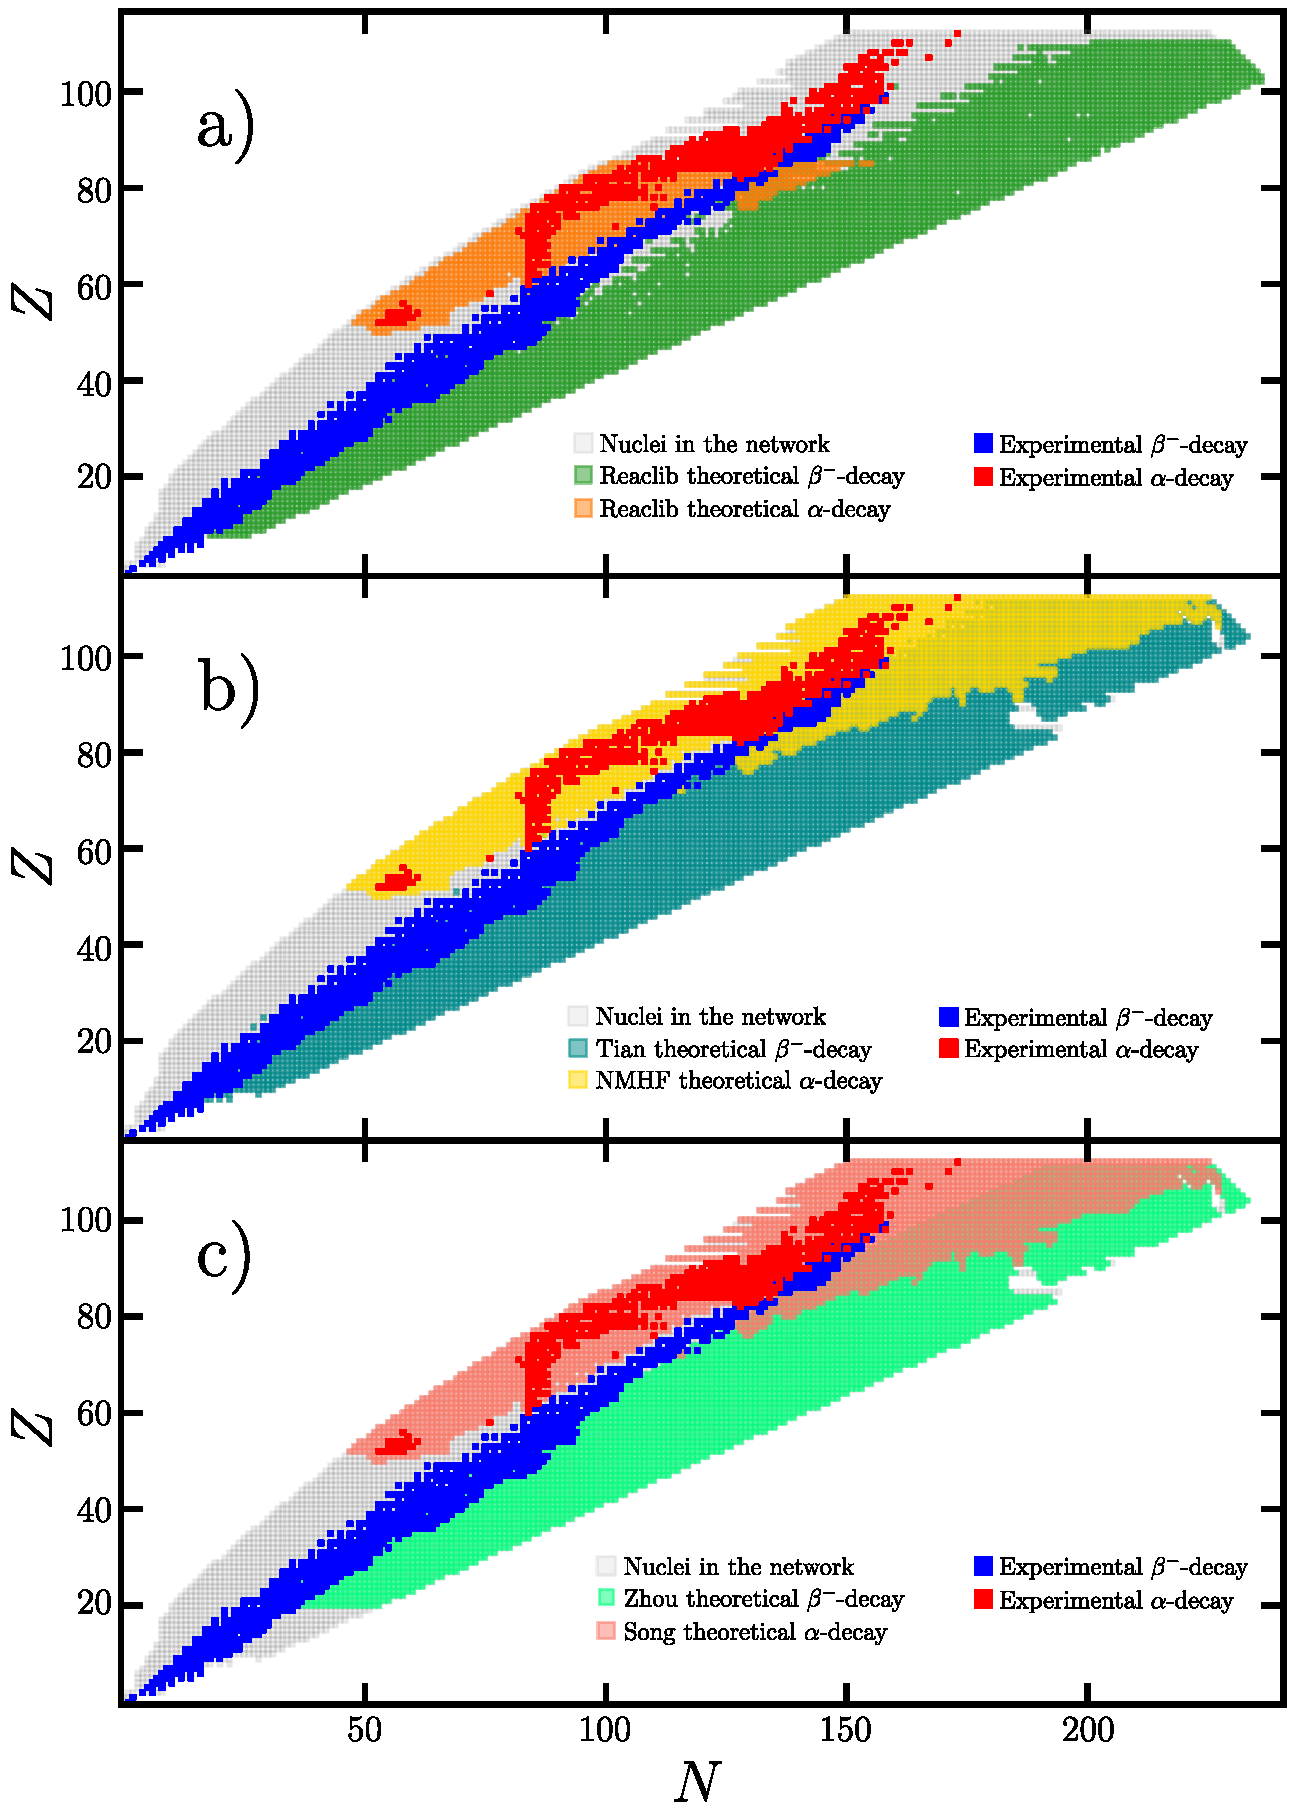
\includegraphics[width=0.95\textwidth]{Figures/Ranges.pdf}
  \caption{Regions of the nuclear chart with measured $\alpha$- and $\beta^-$-decay rates, with theoretical rates in ReacLib, and covered by the empirical formulae. The grey area is the full network. Taken from Ref.~\cite{hernandez_porras_features_2027}.}
  \label{fig:rate_coverage}
\end{figure}

\begin{figure}[t]
  \centering
  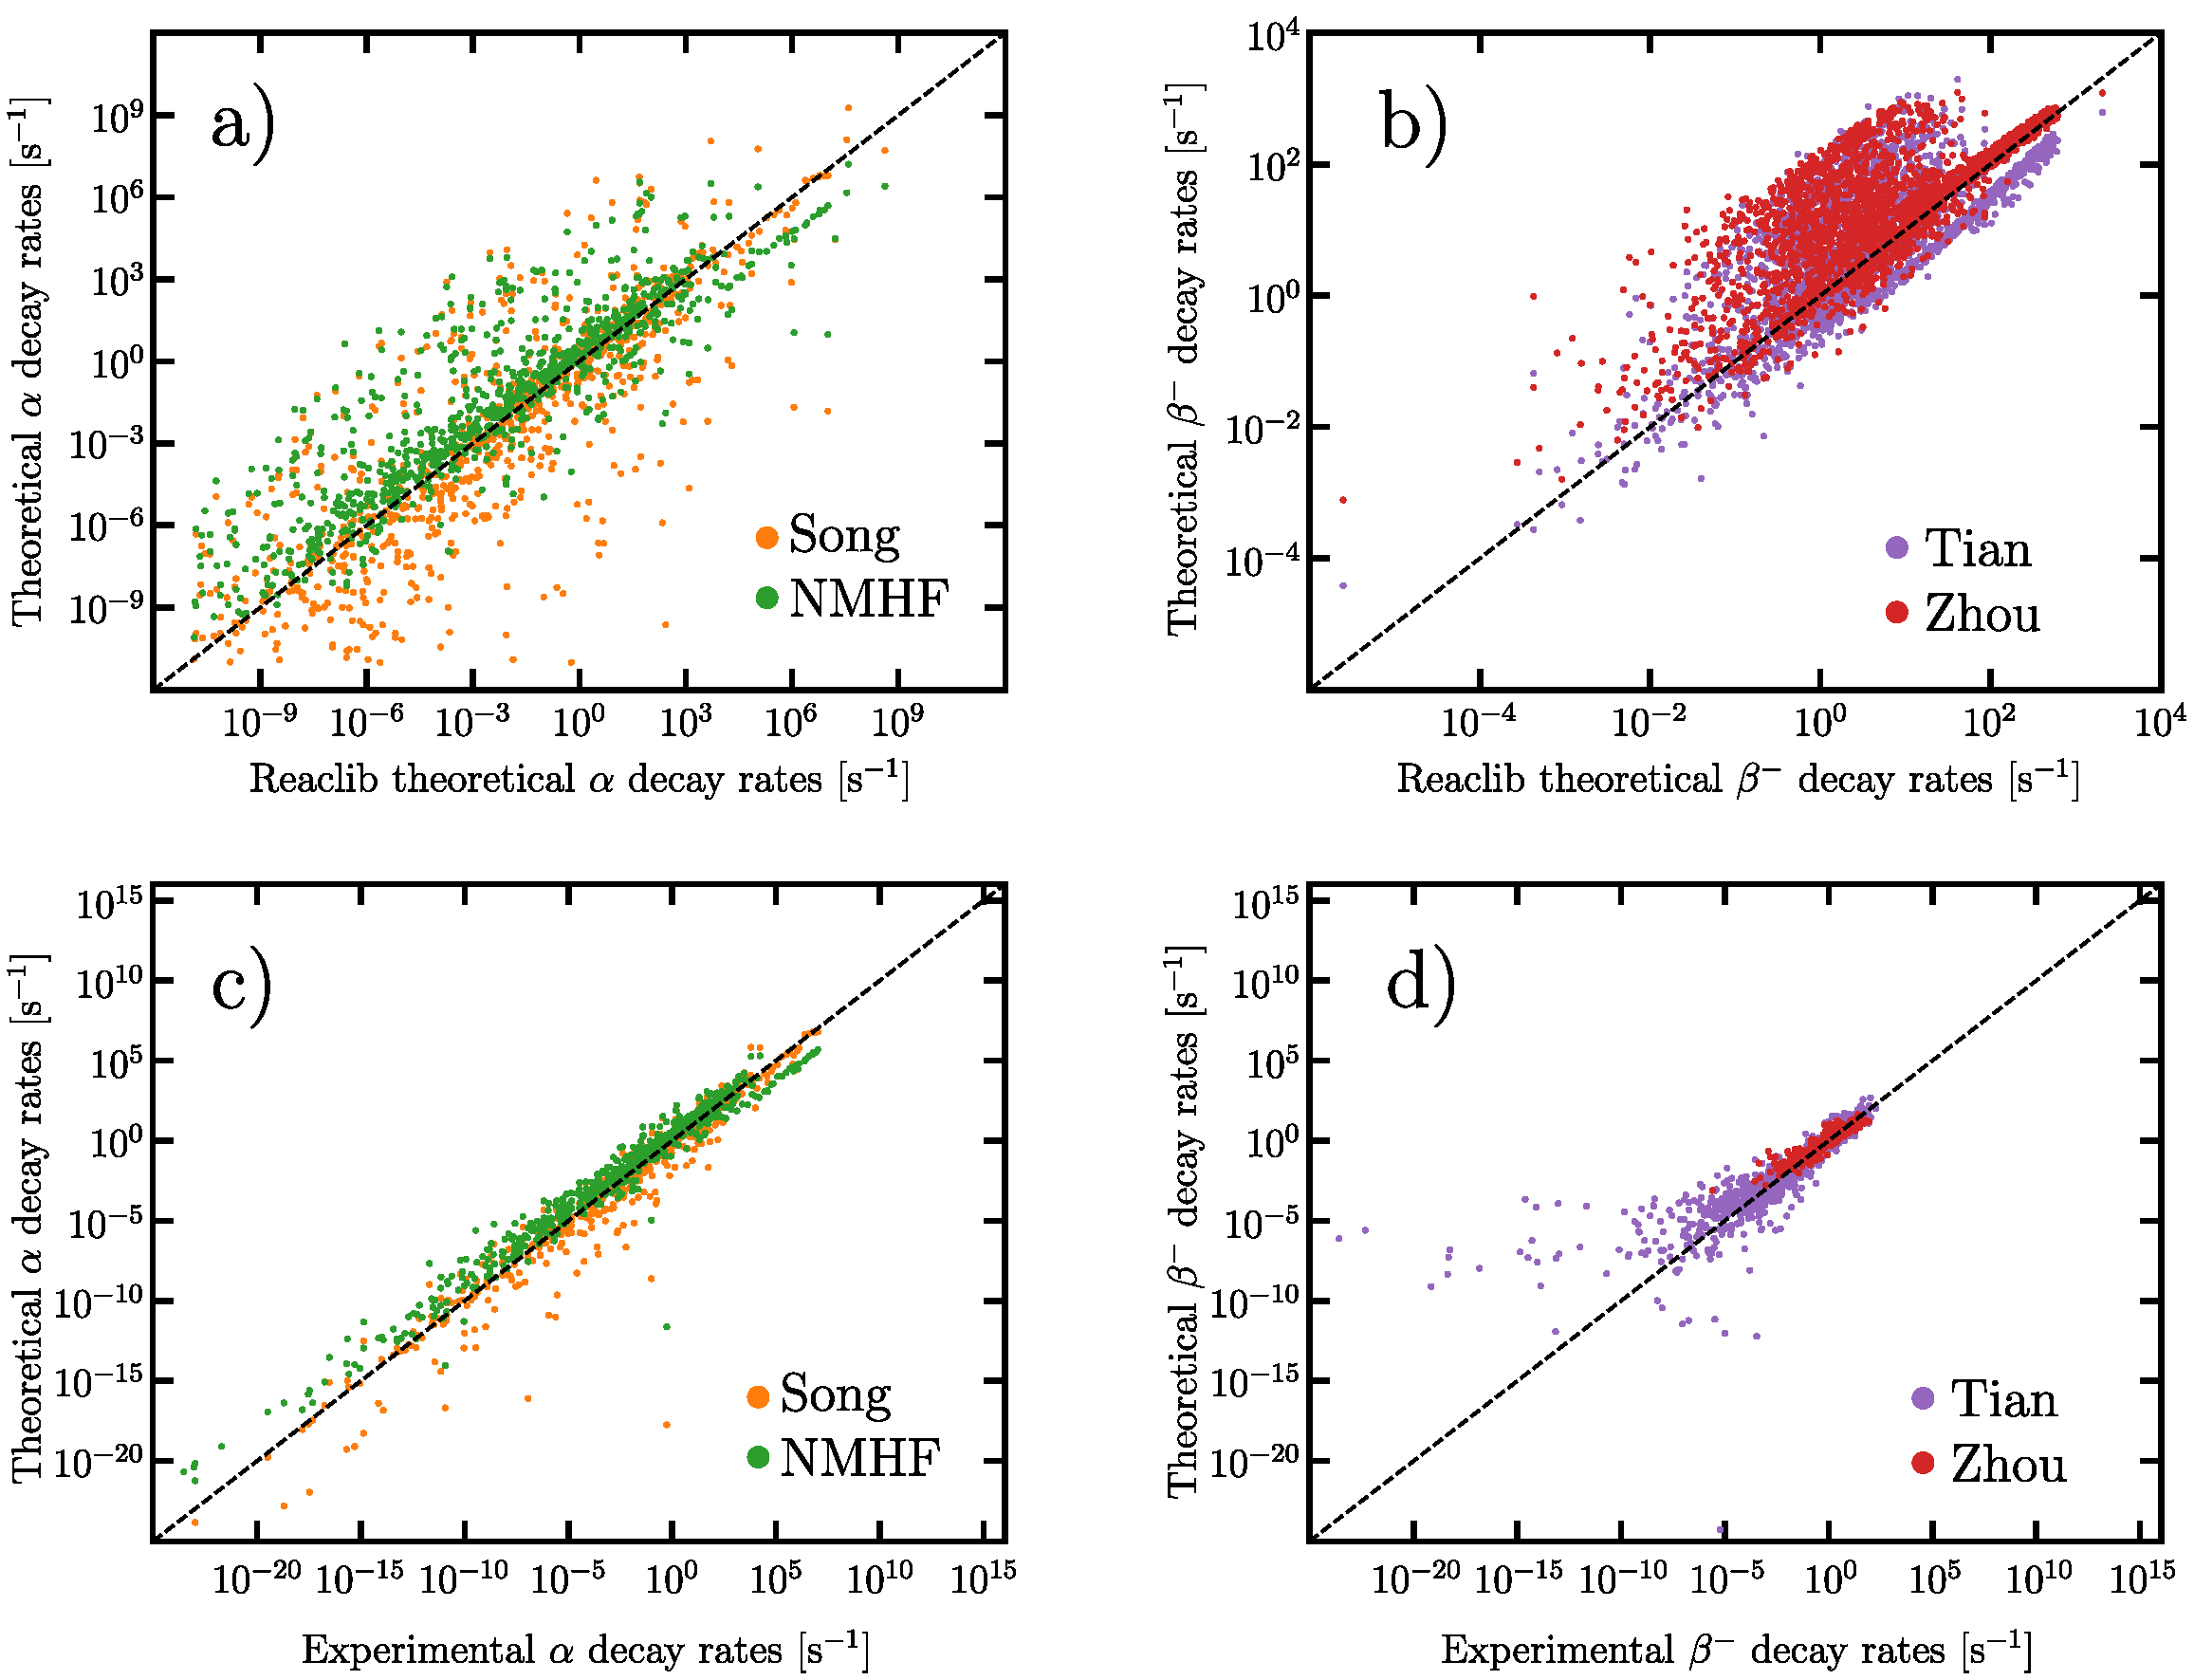
\includegraphics[width=0.95\textwidth]{Figures/Comparison_decay_rates.pdf}
  \caption{Decay rates predicted by the empirical formulae compared with the theoretical rates of ReacLib (top) and with the measured rates (bottom), for $\alpha$ decay (left) and $\beta^-$ decay (right). Taken from Ref.~\cite{hernandez_porras_features_2027}.}
  \label{fig:rate_comparison}
\end{figure}

\subsection{Campaign design and execution}\label{sec:methods_campaign}

Each of the three rate sets was run for the 512 trajectories, 1536 network calculations in total, on the Hypatia high-performance computing cluster of Universidad de los Andes, with one processor core per run.
For each set the rate libraries are first merged by WinNet into a single prepared network, which every run of the set then reads.
This guarantees that the 512 runs of a set use identical nuclear input, and it provides the assembled rates, $Q$-values and neutrino fractions from which the heating is later computed.
A provenance record is stored with every set: the checksum of the parameter template, the checksum of the WinNet executable, the rate library and the fission option.

The runs of a set are numbered in order of increasing $Y_{e,0}$, so a given run number is the same trajectory in the three sets.
All the comparisons of this thesis exploit this pairing.
A ratio between two prescriptions is always the ratio of two calculations that share the trajectory and every nuclear input except the theoretical decay rates, and the spread of such ratios over the ensemble measures how the sensitivity to the decay rates depends on the thermodynamic conditions.